\chapter{Results}
\label{chap:results}

% Qualitative first, as is the way in EDS.
% 	- spectrum calibrated, 5-30 kV
% 	- one plot for all
% 	- Look at energy scale for all results. How does the peaks deviate with the Ga As calibration?
% 	- Cu tape (give type) is not good as a Cu reference.
% 	- The stub is not Fe as expected, but Al. Makes sence, since steel is alloys and is magnetic.

% Quantitative
% 	- initial
% 	- background
% 	- peak fitting


\section{Introduction}
\label{sec:results:intro}
The results are presented in this chapter.
First qualitative then quantitative results are presented.
All the spectra taken were qualitatively analyzed.
The spectrum from the GaAs bulk wafer taken on 30 kV is shown in \cref{fig:GaAs30kV_HS}.
This plot was made with HyperSpy, which utilize Matplotlib for plotting.
The plotting method in HyperSpy can add where the theoretical peak centers are.
The lines added also show an estimate of the weight of the peak.


% add figure figures/GaAs30kV_HS.png
\begin{figure}
    \centering
    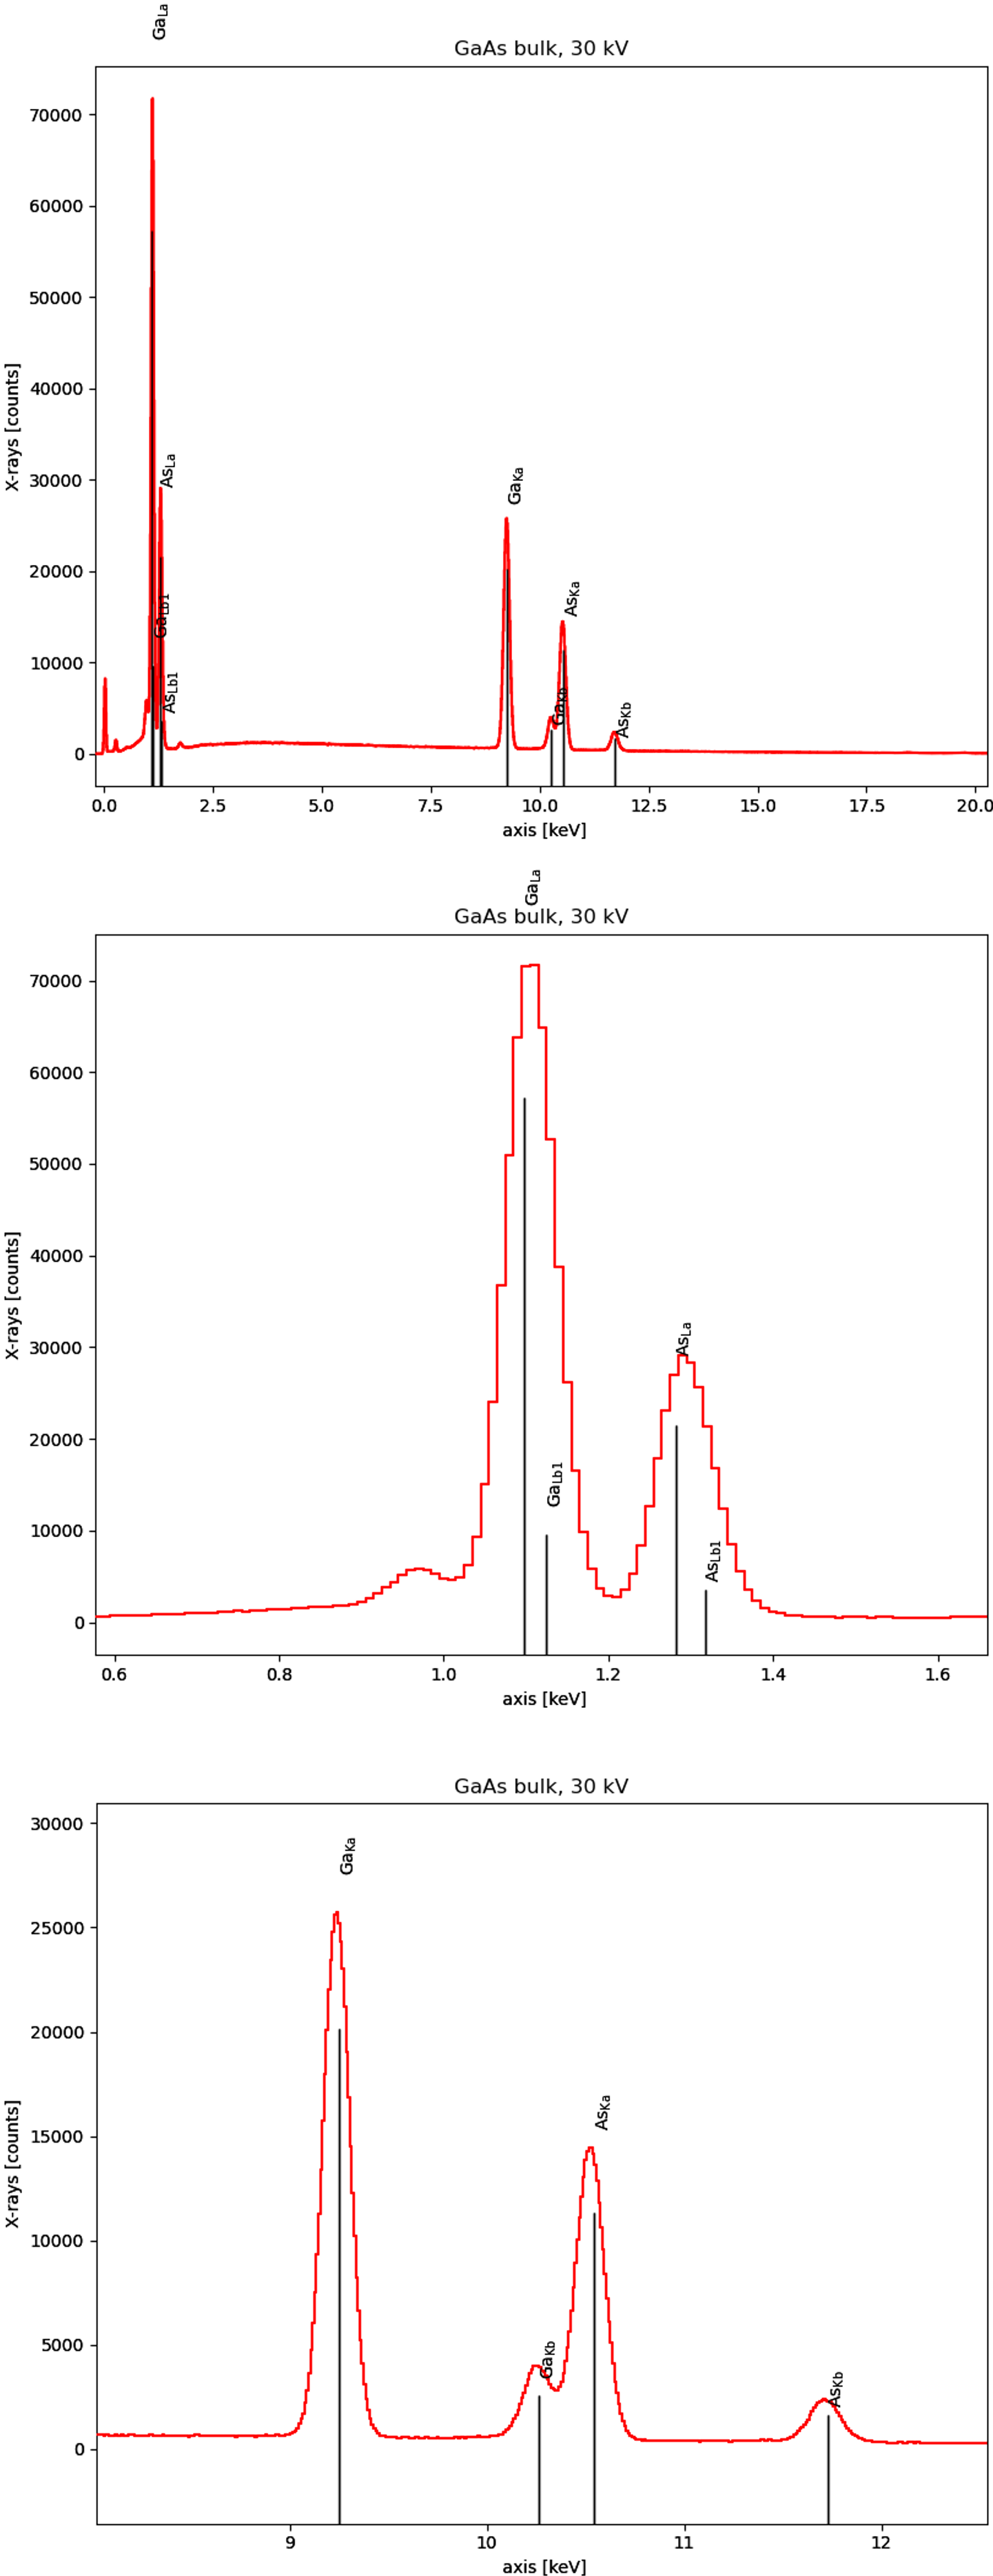
\includegraphics[width=0.45\textwidth]{figures/GaAs30kV_HS.png}
    \caption{
        The GaAs spectrum taken at 30 kV.
        This plot was made with HyperSpy, which use Matplotlib.
        The theoretical peak centers are added as lines.
        The first plot is the whole spectrum, the second is zoomed in on the L-peaks and the last is zoomed in on the K-peaks.
        This plot has the calibration from AZtec, and it is clear that the peak positions are not correct.
    }
    \label{fig:GaAs30kV_HS}
\end{figure}



\section{Qualitative results}
\label{sec:results:qualitative}

\cref{fig:results:Spectra_Al} to \cref{fig:Spectra_Si} shows the plotly spectra for the six sample parts.
The plot is available as an interactive HTML plot on the GitHub repository.
\brynjar{Upload the HTML files to the GitHub repository.}
The calibration used in these spectra is based on the calibration of Ga and As from the GaAs bulk wafer.
The y-axis is normalized to the highest peak value in each spectrum.
When doing the qualitative analysis, it became clear that the FIB stub was not made of Fe as expected, but rather of Al.
Another discovery was that the Cu-tape does not give a good Cu signal.


% figures of the spectras

% figure Spectra_Al.png
\begin{figure}
    \centering
    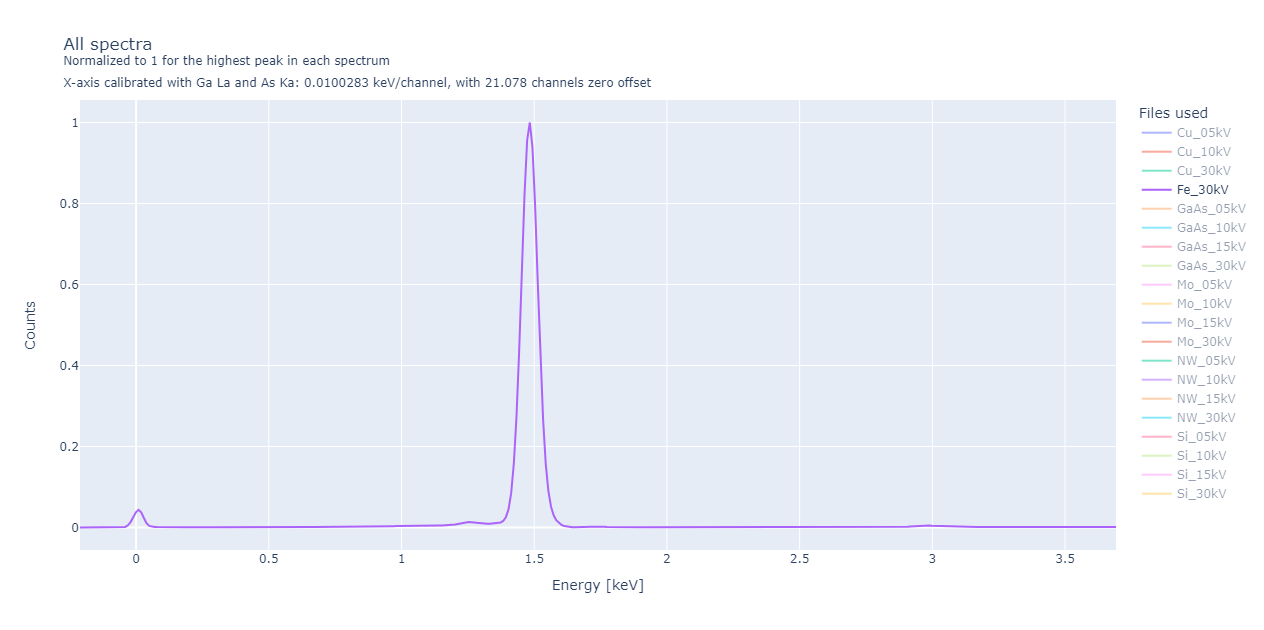
\includegraphics[width=0.70\textwidth]{figures/Spectra_Al.png}
    \caption{
        The spectra of the Al sample part.
        This was expected to be Fe, thus the label is wrong.
        The peak at 1.48 keV is the Al K$\alpha$ peak.
    }
    \label{fig:results:Spectra_Al}
\end{figure}

% figure Spectra_Cu.png
\begin{figure}
    \centering
    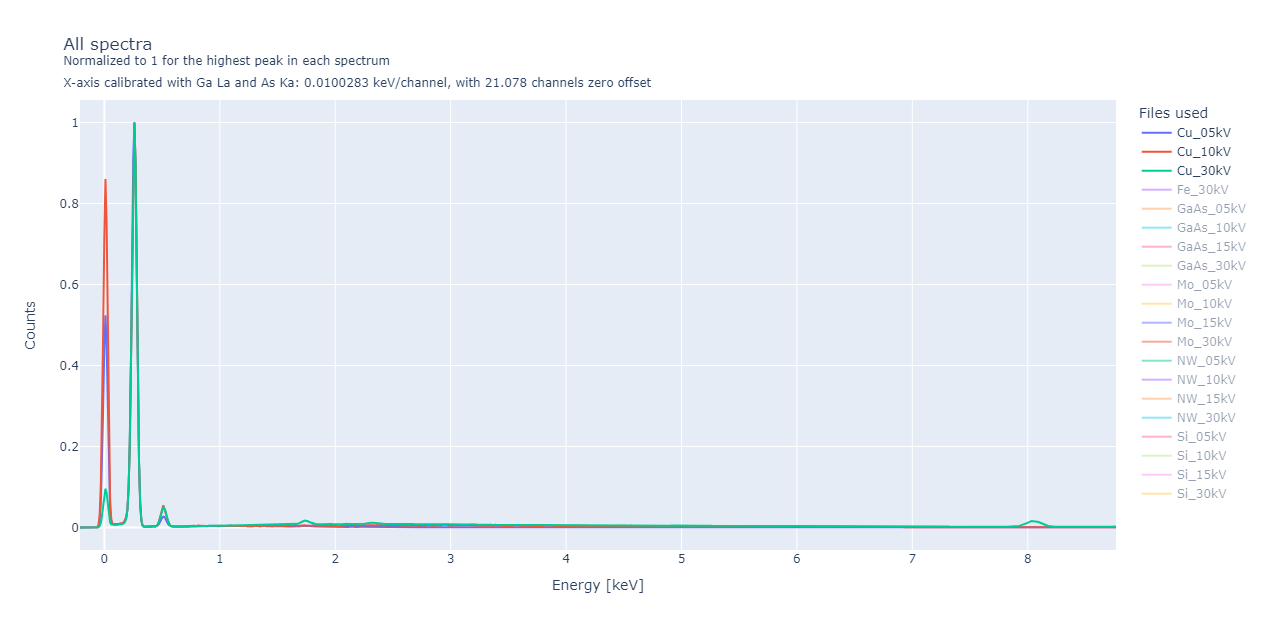
\includegraphics[width=0.70\textwidth]{figures/Spectra_Cu.png}
    \label{fig:Spectra_Cu}
    \caption{
        The spectra of the Cu sample part.
        The Cu sample was Cu-tape from the lab, but the Cu K$\beta$ peak is only barely visible at the 30 kV spectrum.
        The highest peak in all three spectra is at 0.260 keV, which is the C K$\alpha$ peak, slightly off from the expected 0.277 keV.
    }
\end{figure}

% figure Spectra_GaAs.png
\begin{figure}
    \centering
    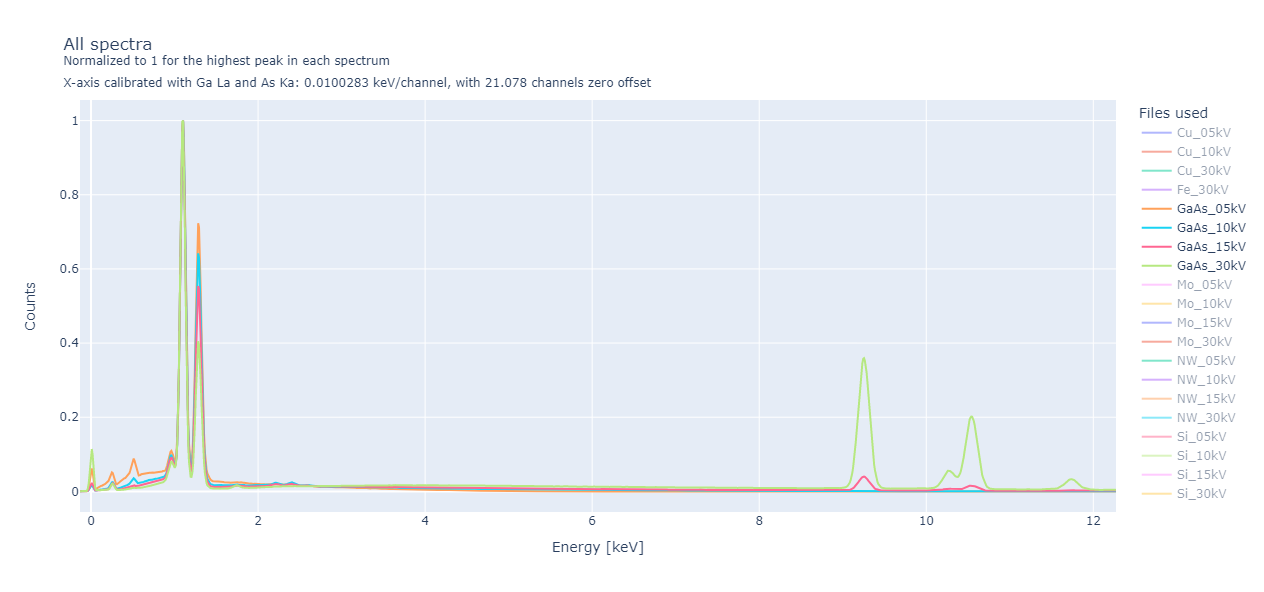
\includegraphics[width=0.70\textwidth]{figures/Spectra_GaAs.png}
    \label{fig:Spectra_GaAs}
    \caption{
        The spectra of the GaAs sample part.
        Both the K-peaks and the L-peaks of Ga and As are visible.
        There is a peak at 0.511 keV, which is the O K$\alpha$ peak.
        There is a peak at 0.260 keV, which is the C K$\alpha$ peak.
    }
\end{figure}

% figure Spectra_Mo.png
\begin{figure}
    \centering
    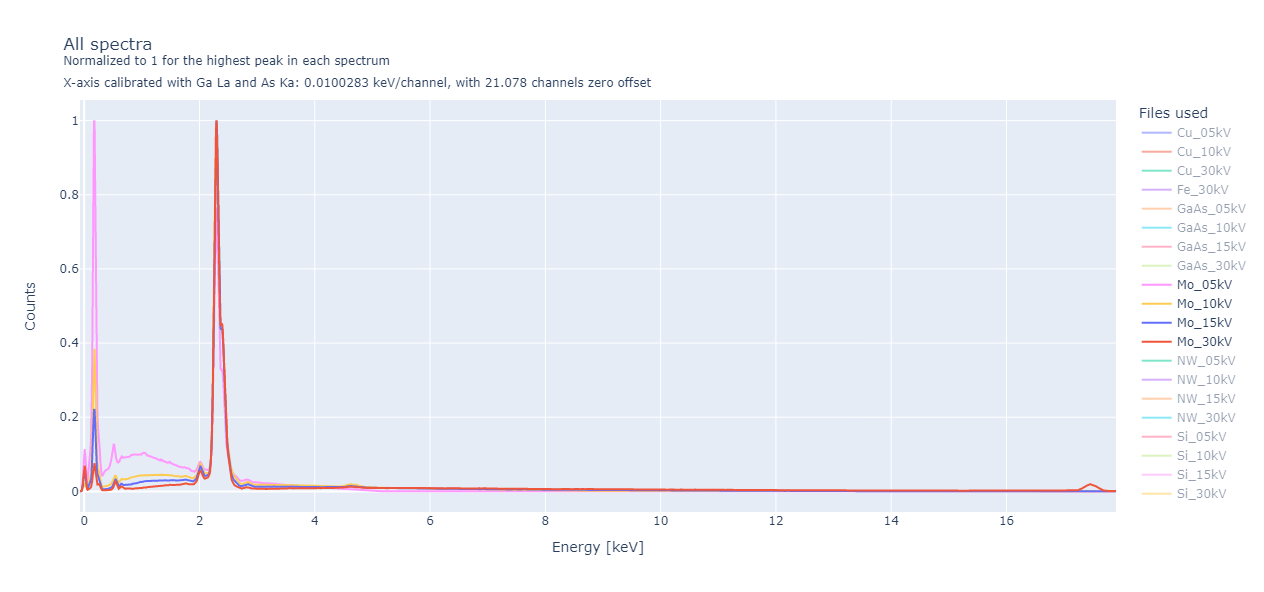
\includegraphics[width=0.70\textwidth]{figures/Spectra_Mo.png}
    \label{fig:Spectra_Mo}
    \caption{
        The spectra of the Mo sample part.
        The Mo K$\alpha$ peak at 17.47 keV is barely visible at the 30 kV spectrum, and has a high noise level.
        The high dobble peak is Mo L$\alpha$ at 2.29 keV and Mo L$\beta$ at 2.39 keV.
    }
\end{figure}

% figure Spectra_NW.png
\begin{figure}
    \centering
    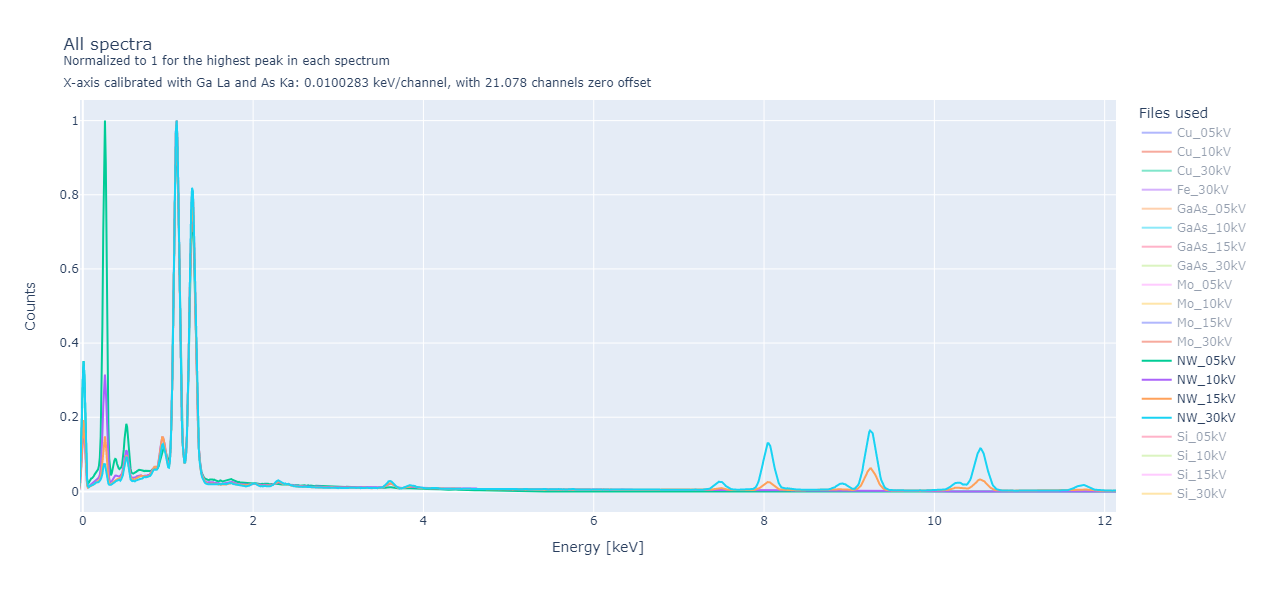
\includegraphics[width=0.70\textwidth]{figures/Spectra_NW.png}
    \label{fig:Spectra_NW}
    \caption{
        The spectra of the nanowire sample part.
        This spectrum have the most peaks, and contains Ga, As, Cu, Sb (? at 3.6 keV), Mo, C, and O.
    }
\end{figure}

% figure Spectra_Si.png
\begin{figure}
    \centering
    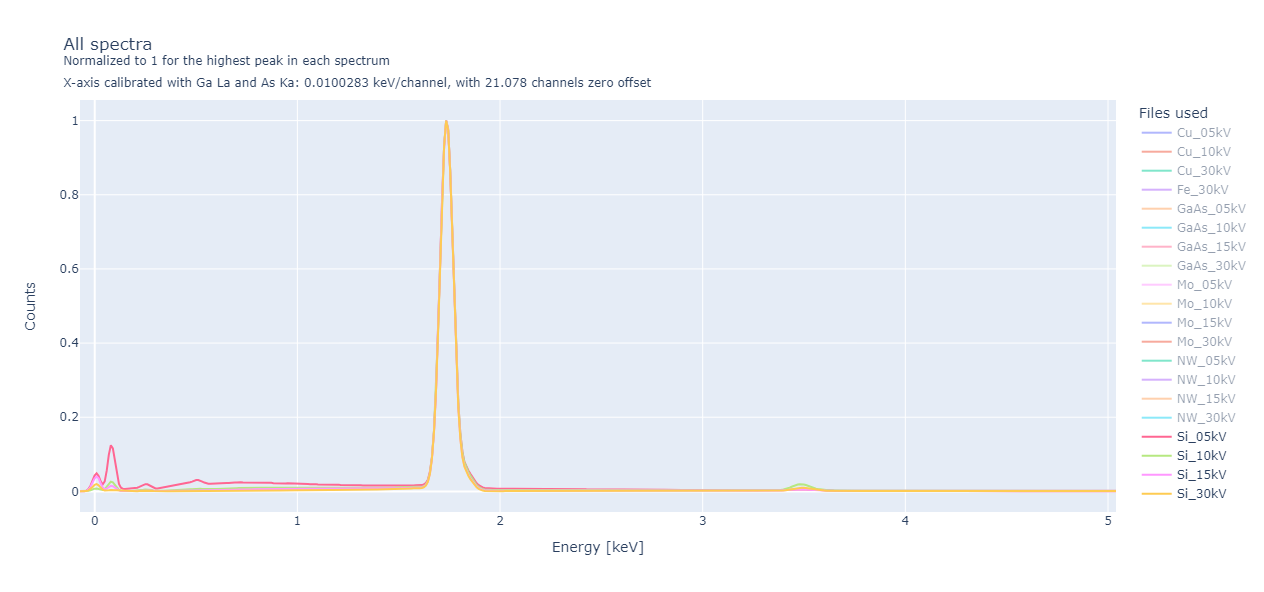
\includegraphics[width=0.70\textwidth]{figures/Spectra_Si.png}
    \label{fig:Spectra_Si}
    \caption{
        The spectra of the pure Si wafer sample part.
        All four spectra have one large peak at 1.73 keV, which is the Si K$\alpha$ peak.
        The four spectra also have a small peak at 3.48 keV, which is not identified.
    }
\end{figure}

\subsection{Calibration}
\label{sec:results:qualitative:calibration}

Different calibrations were explored.
The initial calibration is the one from AZtec, and is the one used in the spectra in \cref{fig:GaAs30kV_HS}.
This calibration has a left shift for the L-peaks and a right shift for the K-peaks.
The second type of calibration is the one given by the model fit in HyperSpy.
The third type is from the self made model fit, using the distance between two high intensity and far apart peaks to calibrate the energy scale.
All three types are given in \ref{tab:results:calibrations}.
The deviations are a few percent, and the accuracy of the different calibrations give on spesific peaks are given in \cref{tab:results:calibration-peak-accuracy}.
Here accuracy is the difference between the theoretical peak position and the peak center in the spectrum, given in percent.

% dispersion and offset table
% Calibration values
% chapter Results
\begin{table}[ht]
    \centering
    \caption{
        Different calibration values.
        The AZtec calibration is reffered to as the uncalibrated value.
        The dispersion is calculated with \cref{eq:theory:calibration:dispersion}.
        The offset is calculated with \cref{eq:theory:calibration:offset}.
        The own calibration was done on Ga L$_\alpha$ and As K$_\alpha$ from the 30 kV measurement on the GaAs wafer.
        The HyperSpy cailbration was done by making a model and fitting it to the data on the 30 kV GaAs spectrum.
    }
    \label{tab:results:calibrations}
    % \begin{tabular}{m{4cm} m{2cm} m{2cm}}
    \begin{tabular}{ccc}
        Calibration method & Dispersion,   & Zero offset \\
                           & [keV/channel] & [channels]  \\
        \hline
        AZtec              & 0.01          & 20          \\
        HyperSpy           & 0.010028      & 21.0787     \\
        Own calibration    & 0.010030      & 21.127
    \end{tabular}
\end{table}


% calibration peak accuracy table
% table with peak accuracy

\begin{table}[p]
    \centering
    \caption{
        % TODO: give the peak accuracy in ev, not percent. Or eV and percent?
        Peak accuracy of the different calibration methods on 30 kV spectra: NW, Mo, Si, Al, Cu. % TODO: reformulate
        The other acceleration voltages gave similar results.
        The accuracy here is the deviation from the theoretical peak to the measured peak.
        The percentage deviation is also given.
        The measured peak is the fitted center of the peak.
        % discussion: The Mo L$\alpha$ deviates much because the peak is not well fitted.
        % The C K$\alpha$ is fitted well, but deviates much more than all the other peaks.
        The self-made calibration was done on two spectra: GaAs and Mo. % discussion: Mo is more far apart than GaAs.
        % One was done on Ga L$\alpha$ and As K$\alpha$ from the 30 kV measurement on the GaAs wafer.
        % The other was done on the more far apart peaks Mo L$\alpha$ and Mo K$\alpha$ from the 30 kV measurement on the Mo wafer.
        The HyperSpy calibration was done on the GaAs spectrum.
        At the bottom the RMS of the deviation in the column is given.
    }
    \label{tab:results:calibration-peak-accuracy}
    \begin{tabular}{cccccc}
        Peak         & Theoretical & AZtec                 & HyperSpy              & Ga L$\alpha$ \& As K$\alpha$ & Mo L$\alpha$ \& Mo K$\alpha$ \\
                     & [keV]       & [eV]                  & [eV]                  & [eV]                         & [eV]                         \\
        \hline
        As L$\alpha$ & 1.2819      & 12.8,\,\,\,    1.0\%  & 5.6,\,\,\,    0.4\%   & 5.4,\,\,\,    0.4\%          & 7.2,\,\,\,    0.6\%          \\
        As K$\alpha$ & 10.5436     & -21.3,\,\,\,   -0.2\% & -2.7,\,\,\,   -0.0\%  & -1.1,\,\,\,   -0.0\%         & 9.8,\,\,\,    0.1\%          \\
        Ga L$\alpha$ & 1.098       & 11.5,\,\,\,    1.0\%  & 3.8,\,\,\,    0.3\%   & 3.5,\,\,\,    0.3\%          & 5.1,\,\,\,    0.5\%          \\
        Ga K$\alpha$ & 9.2517      & -14.2,\,\,\,   -0.2\% & 0.9,\,\,\,    0.0\%   & 2.2,\,\,\,    0.0\%          & 11.9,\,\,\,    0.1\%         \\
        Cu L$\alpha$ & 0.9295      & 16.4,\,\,\,    1.8\%  & 8.3,\,\,\,    0.9\%   & 8.0,\,\,\,    0.9\%          & 9.4,\,\,\,    1.0\%          \\
        Cu K$\alpha$ & 8.0478      & -9.2,\,\,\,   -0.1\%  & 2.5,\,\,\,    0.0\%   & 3.7,\,\,\,    0.0\%          & 12.1,\,\,\,    0.2\%         \\
        Mo K$\alpha$ & 17.4793     & -56.8,\,\,\,   -0.3\% & -18.8,\,\,\,   -0.1\% & -15.8,\,\,\,   -0.1\%        & 1.9,\,\,\,    0.0\%          \\
        Mo L$\alpha$ & 2.2932      & 24.0,\,\,\,    1.0\%  & 19.7,\,\,\,    0.9\%  & 19.7,\,\,\,    0.9\%         & 22.5,\,\,\,    1.0\%         \\
        Si K$\alpha$ & 1.7397      & 2.9,\,\,\,    0.2\%   & -3.0,\,\,\,   -0.2\%  & -3.2,\,\,\,   -0.2\%         & -1.0,\,\,\,   -0.1\%         \\
        Al K$\alpha$ & 1.4865      & 3.0,\,\,\,    0.2\%   & -3.7,\,\,\,   -0.2\%  & -3.9,\,\,\,   -0.3\%         & -1.9,\,\,\,   -0.1\%         \\
        Cu K$\alpha$ & 8.0478      & -9.3,\,\,\,   -0.1\%  & 2.4,\,\,\,    0.0\%   & 3.5,\,\,\,    0.0\%          & 11.9,\,\,\,    0.1\%         \\
        C K$\alpha$  & 0.2774      & -8.2,\,\,\,   -3.0\%  & -18.3,\,\,\,   -6.6\% & -18.7,\,\,\,   -6.7\%        & -17.9,\,\,\,   -6.5\%        \\
        \hline
        RMS  [eV]    &             & 14.75                 & 4.62                  & 4.55                         & 9.57
    \end{tabular}
\end{table}



\section{Quantitative results}
\label{sec:results:quantification}


\subsection{Initial quantification}
\label{sec:results:initial_quantification}
% How accurate it the out-of-the-box quantification in AZtec and HyperSpy?

The initial quantification was done on the data from the GaAs wafer in AZtec and in HyperSpy as out-of-the-box as possible.
The results are presented in \cref{tab:initial_quantification}.
The wafer is a 1:1 alloy of gallium and arsenic, so the atomic percent of Ga and As should be 50\% and 50\% respectively.

% initial quantification
% chapter Results
\begin{table}[ht]
    \centering
    \caption{
        Initial quantification of the GaAs wafer.
        The ratio in the wafer is 1:1, so the correct ratio is 50\% and 50\%, because the results are in atomic percent.
        \brynjar{Put in the actual results here. Use both HyperSpy linear and model fitted results?}
    }
    \label{tab:initial_quantification}
    \begin{tabular}{m{1.5cm} m{1.5cm} m{1.5cm} m{1.5cm} m{1.5cm}}
        $V_\textnormal{acc}$ & AZtec &       & HyperSpy &       \\
                             & Ga    & As    & Ga       & As    \\
        \hline
        5 kV                 & 50 \% & 50 \% & 50 \%    & 50 \% \\
        10 kV                & 50 \% & 50 \% & 50 \%    & 50 \% \\
        15 kV                & 50 \% & 50 \% & 50 \%    & 50 \% \\
        30 kV                & 50 \% & 50 \% & 50 \%    & 50 \%
    \end{tabular}
\end{table}
